

\tikzset{every picture/.style={line width=0.75pt}} %set default line width to 0.75pt        

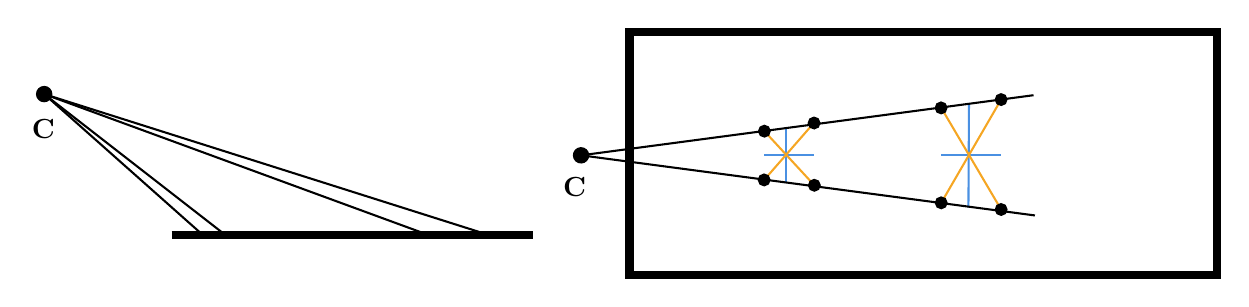
\begin{tikzpicture}[x=0.75pt,y=0.75pt,yscale=-1,xscale=1]
%uncomment if require: \path (0,142); %set diagram left start at 0, and has height of 142

%Straight Lines [id:da6840514143989631] 
\draw [color={rgb, 255:red, 74; green, 144; blue, 226 }  ,draw opacity=1 ]   (366.4,69.04) -- (390.44,69.04) ;
%Straight Lines [id:da9689027017272559] 
\draw [color={rgb, 255:red, 74; green, 144; blue, 226 }  ,draw opacity=1 ]   (377.02,82.13) -- (377.02,55.88) ;
%Straight Lines [id:da8683032061954556] 
\draw [color={rgb, 255:red, 74; green, 144; blue, 226 }  ,draw opacity=1 ]   (451.65,69.04) -- (480.52,69.04) ;
%Straight Lines [id:da6934594327602702] 
\draw [color={rgb, 255:red, 74; green, 144; blue, 226 }  ,draw opacity=1 ]   (464.75,94.04) -- (465.02,44.04) ;
%Straight Lines [id:da7261021710957941] 
\draw [color={rgb, 255:red, 245; green, 166; blue, 35 }  ,draw opacity=1 ]   (480.5,42.14) -- (451.64,91.89) ;
%Straight Lines [id:da37992799055918147] 
\draw [color={rgb, 255:red, 245; green, 166; blue, 35 }  ,draw opacity=1 ]   (451.58,46) -- (480.5,95.1) ;
%Straight Lines [id:da15457235634391941] 
\draw [color={rgb, 255:red, 245; green, 166; blue, 35 }  ,draw opacity=1 ]   (389.38,54.43) -- (366.33,80.86) ;
%Straight Lines [id:da05878950535382432] 
\draw [color={rgb, 255:red, 245; green, 166; blue, 35 }  ,draw opacity=1 ]   (366.45,57.36) -- (390.5,83.43) ;
%Straight Lines [id:da045550454885305736] 
\draw [line width=3]    (80.9,107.5) -- (254.9,107.5) ;
%Shape: Circle [id:dp8549507101465224] 
\draw  [fill={rgb, 255:red, 0; green, 0; blue, 0 }  ,fill opacity=1 ] (16,39.5) .. controls (16,37.59) and (17.54,36.05) .. (19.45,36.05) .. controls (21.36,36.05) and (22.9,37.59) .. (22.9,39.5) .. controls (22.9,41.41) and (21.36,42.95) .. (19.45,42.95) .. controls (17.54,42.95) and (16,41.41) .. (16,39.5) -- cycle ;
%Straight Lines [id:da09684243305909856] 
\draw    (19.45,39.5) -- (94.9,106.5) ;
%Straight Lines [id:da4476141598512392] 
\draw    (19.45,39.5) -- (106.9,107.5) ;
%Straight Lines [id:da5555101325179832] 
\draw    (19.45,39.5) -- (204.9,107.5) ;
%Straight Lines [id:da06573307117836547] 
\draw    (19.45,39.5) -- (230.9,106.5) ;
%Shape: Circle [id:dp3195203497272404] 
\draw  [fill={rgb, 255:red, 0; green, 0; blue, 0 }  ,fill opacity=1 ] (274.67,69.08) .. controls (274.62,67.18) and (276.13,65.6) .. (278.04,65.55) .. controls (279.94,65.51) and (281.52,67.02) .. (281.57,68.92) .. controls (281.61,70.83) and (280.1,72.41) .. (278.2,72.45) .. controls (276.29,72.49) and (274.71,70.99) .. (274.67,69.08) -- cycle ;
%Straight Lines [id:da25083036265050096] 
\draw    (278.12,69) -- (496.79,97.97) ;
%Straight Lines [id:da6083860800665152] 
\draw    (278.12,69) -- (496.1,40.04) ;
%Shape: Rectangle [id:dp031034421219254926] 
\draw  [line width=3]  (301.4,9.5) -- (584.4,9.5) -- (584.4,126.5) -- (301.4,126.5) -- cycle ;
%Shape: Circle [id:dp2988386895287467] 
\draw  [fill={rgb, 255:red, 0; green, 0; blue, 0 }  ,fill opacity=1 ] (363.85,57.42) .. controls (363.81,55.99) and (364.95,54.8) .. (366.39,54.76) .. controls (367.82,54.73) and (369.01,55.87) .. (369.05,57.3) .. controls (369.08,58.74) and (367.94,59.93) .. (366.51,59.96) .. controls (365.07,60) and (363.88,58.86) .. (363.85,57.42) -- cycle ;
%Shape: Circle [id:dp49087747494377276] 
\draw  [fill={rgb, 255:red, 0; green, 0; blue, 0 }  ,fill opacity=1 ] (363.73,80.92) .. controls (363.69,79.48) and (364.83,78.29) .. (366.27,78.26) .. controls (367.7,78.23) and (368.89,79.36) .. (368.93,80.8) .. controls (368.96,82.23) and (367.82,83.42) .. (366.39,83.46) .. controls (364.95,83.49) and (363.76,82.35) .. (363.73,80.92) -- cycle ;
%Shape: Circle [id:dp3291682457892863] 
\draw  [fill={rgb, 255:red, 0; green, 0; blue, 0 }  ,fill opacity=1 ] (387.79,53.49) .. controls (387.75,52.06) and (388.89,50.87) .. (390.32,50.84) .. controls (391.76,50.8) and (392.95,51.94) .. (392.98,53.37) .. controls (393.02,54.81) and (391.88,56) .. (390.44,56.03) .. controls (389.01,56.07) and (387.82,54.93) .. (387.79,53.49) -- cycle ;
%Shape: Circle [id:dp598750640317177] 
\draw  [fill={rgb, 255:red, 0; green, 0; blue, 0 }  ,fill opacity=1 ] (387.91,83.49) .. controls (387.87,82.05) and (389.01,80.86) .. (390.44,80.83) .. controls (391.88,80.79) and (393.07,81.93) .. (393.1,83.37) .. controls (393.14,84.8) and (392,85.99) .. (390.56,86.03) .. controls (389.13,86.06) and (387.94,84.92) .. (387.91,83.49) -- cycle ;
%Shape: Circle [id:dp3156912690396848] 
\draw  [fill={rgb, 255:red, 0; green, 0; blue, 0 }  ,fill opacity=1 ] (449.04,91.95) .. controls (449.01,90.51) and (450.14,89.32) .. (451.58,89.29) .. controls (453.02,89.26) and (454.21,90.39) .. (454.24,91.83) .. controls (454.27,93.26) and (453.13,94.45) .. (451.7,94.49) .. controls (450.26,94.52) and (449.07,93.38) .. (449.04,91.95) -- cycle ;
%Shape: Circle [id:dp0381257221295519] 
\draw  [fill={rgb, 255:red, 0; green, 0; blue, 0 }  ,fill opacity=1 ] (448.99,46.21) .. controls (448.95,44.77) and (450.09,43.58) .. (451.53,43.55) .. controls (452.96,43.52) and (454.15,44.65) .. (454.18,46.09) .. controls (454.22,47.53) and (453.08,48.72) .. (451.65,48.75) .. controls (450.21,48.78) and (449.02,47.65) .. (448.99,46.21) -- cycle ;
%Shape: Circle [id:dp4047969379608699] 
\draw  [fill={rgb, 255:red, 0; green, 0; blue, 0 }  ,fill opacity=1 ] (477.91,42.2) .. controls (477.87,40.76) and (479.01,39.57) .. (480.44,39.54) .. controls (481.88,39.51) and (483.07,40.64) .. (483.1,42.08) .. controls (483.14,43.51) and (482,44.7) .. (480.56,44.74) .. controls (479.13,44.77) and (477.94,43.63) .. (477.91,42.2) -- cycle ;
%Shape: Circle [id:dp5781527725767942] 
\draw  [fill={rgb, 255:red, 0; green, 0; blue, 0 }  ,fill opacity=1 ] (477.91,95.16) .. controls (477.87,93.72) and (479.01,92.53) .. (480.44,92.5) .. controls (481.88,92.46) and (483.07,93.6) .. (483.1,95.04) .. controls (483.14,96.47) and (482,97.66) .. (480.56,97.69) .. controls (479.13,97.73) and (477.94,96.59) .. (477.91,95.16) -- cycle ;

% Text Node
\draw (12,50.05) node [anchor=north west][inner sep=0.75pt]   [align=left] {$\displaystyle \mathbf{C}$};
% Text Node
\draw (268,78.05) node [anchor=north west][inner sep=0.75pt]   [align=left] {$\displaystyle \mathbf{C}$};


\end{tikzpicture}
